\documentclass[11pt,letterpaper]{article}
\usepackage[margin=1in]{geometry}
\usepackage[T1]{fontenc}
\usepackage{lmodern,microtype,amsmath,amssymb,amsthm,mathtools,booktabs,graphicx}
\usepackage[numbers,sort&compress]{natbib}
\usepackage{xcolor}
\usepackage[colorlinks=true,linkcolor=blue!45!black,citecolor=blue!45!black,urlcolor=blue!45!black]{hyperref}
\usepackage{enumitem,fancyhdr}
\setlist{nosep,leftmargin=1.4em}
\setlength{\parskip}{3pt}
\setlength{\parindent}{1.2em}
\setlength{\emergencystretch}{2em}
\pagestyle{fancy}\fancyhf{}\fancyhead[L]{\small Editing What Prediction Forgets}\fancyhead[R]{\small Gupta}\fancyfoot[C]{\thepage}
\newtheorem{theorem}{Theorem}
\newtheorem{proposition}[theorem]{Proposition}
\newtheorem{corollary}[theorem]{Corollary}
\newtheorem{definition}[theorem]{Definition}
\newcommand{\one}{\mathbf{1}}
\newcommand{\TV}{\operatorname{TV}}
\newcommand{\spn}{\operatorname{span}}
\newcommand{\col}{\operatorname{col}}
\newcommand{\rank}{\operatorname{rank}}
\newcommand{\Kset}{\mathcal{K}}
\newcommand{\V}{\mathcal{V}}
\newcommand{\N}{\mathcal{N}}
\newcommand{\D}{\Delta}
\title{\vspace{-1.8em}\textbf{Editing What Prediction Forgets:}\\Support-Constrained Repair of\\Compressed Belief Dynamics}
\author{Shivam Gupta\\Independent Researcher\\\texttt{shivam1720406@gmail.com}}
\date{17 October 2026}
\newcommand{\PartitionRow}{Partition & 120 & 0.346 & 0.397 & 0.997 & 5.3 \\}
\newcommand{\MixtureRow}{Mixture & 120 & 0.233 & --- & 0.999 & 9.0 \\}

\begin{document}
\maketitle
\begin{abstract}
A belief representation can preserve every passive prediction while failing to support a specified edit of that belief. We study this interface for known finite hidden-state models and row-stochastic edits. An edit is implementable on the predictive representation exactly when it preserves predictive equivalence, including equivalence between mixtures of latent states. We turn this classical quotient condition into an audit with three outcomes: accept an edit, retain additional predictive coordinates, or change the edit subject to declared transition restrictions. For a fixed representation, the smallest worst-prior total-variation change is a linear program. For partition representations, we derive a support-constrained block-center formulation and an explicit feasibility obstruction: every source block must have a target block accessible from each of its members. Constructed families exhibit passive dimension two but edit-closed dimension $n$, and unavoidable repair cost $1-1/m$. Independent rational checks cover 574 deterministic cases. Experiments on 240 generated models and 120 sparse-support specifications validate the implementation; 25 sparse-support specifications admit no compatible repair. A stronger mean-aggregate baseline reduces the apparent benefit of optimization, with a remaining mean paired improvement of 0.052 total variation. The result is an executable specification for finite belief edits, rather than evidence that neural activation steering is already certified.
\end{abstract}
\noindent\textbf{Keywords:} predictive representations; belief editing; causal abstraction; stochastic kernels; support constraints; minimax approximation.

\section{Introduction}
A useful world model need not retain every distinction in its latent description. Two beliefs can assign the same probability to every future observation, making their difference irrelevant to passive prediction. The same difference may become relevant after an intervention. This poses an interface question: if a controller receives only the compressed predictive state, can it implement a requested edit without recovering information that the representation has discarded?

Consider latent states $1,2,3$. State 3 predicts the same future as an equal mixture of states 1 and 2. A representation sufficient for prediction can therefore identify the beliefs $e_3$ and $(e_1+e_2)/2$. Now request an edit that sends state 3 to state 1 while leaving the first two states unchanged. The two equivalent inputs require different edited predictions. No deterministic function of their shared representation can satisfy both requests (Figure~\ref{fig:mixture}). Comparing only pairs of individual latent states misses this example: no two individual states need have identical predictive behavior.

This issue concerns a specified intervention and representation together. It does not imply that predictive representations are defective, that every latent distinction should be retained, or that all useful edits are impossible. A full reset to a fixed belief is always compatible. The problem is selective manipulation that depends on distinctions absent from the interface.

The motivation connects two established research strands. Observable operator models and predictive state representations formalize sufficient state through future tests \citep{jaeger2000,littman2001,singh2004}. Causal abstraction asks whether low-level and high-level interventions agree \citep{rubenstein2017,geiger2025}. Recent belief-geometry studies make the connection relevant to interpretability: belief states can be decoded from transformer activations, and interventions on identified subspaces have been tested in pretrained models \citep{shai2024,balcells2026}. A successful probe, however, does not by itself specify which edits descend to the chosen representation.

We give a finite, model-relative audit of that specification. Its mathematical ingredients are classical invariant-subspace and stochastic-approximation tools. The contribution is their integration around \emph{a fixed predictive interface and a requested edit}, including a support-constrained repair problem, a blockwise exact reduction, sharp failure families, and independently checkable computational artifacts. We distinguish these results from claims of a new abstraction theory or a certified neural editing method.

The paper addresses three questions. (1) What must an edit preserve to be well-defined on a predictive belief representation? (2) If it is incompatible, what is the least change required, and can transition restrictions make repair impossible? (3) What do exact examples and computational checks establish about the resulting audit? We answer these questions under explicit finite-model assumptions. Practical deployment additionally requires learning the model and grounding its edits in actual neural or software mechanisms.

\begin{figure}[t]
\centering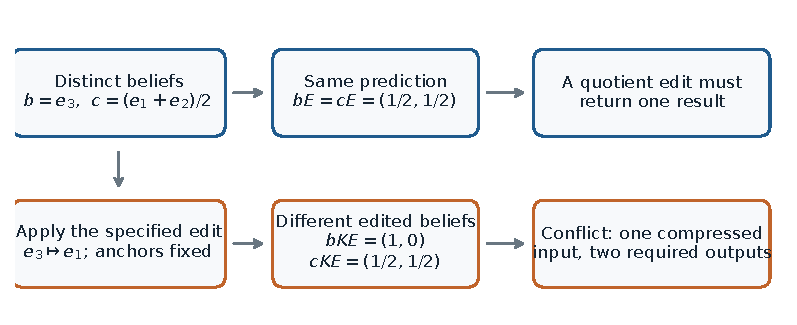
\includegraphics[width=\linewidth]{../figures/01_mixture_obstruction.pdf}
\caption{An incompatible edit on a nonpartition representation. The same compressed belief must be sent to two different predictive outputs. Here $E$ has rows $(1,0),(0,1),(1/2,1/2)$; the example concerns mixtures, even though its individual latent rows are distinct.}\label{fig:mixture}
\end{figure}

\section{Related work and the scope of the contribution}
\paragraph{Predictive state and linear realizations.}
The future-test representation used below is standard in observable operator models and predictive state representations \citep{jaeger2000,littman2001,singh2004}. Backward-space closure, finite equivalence tests, and linear minimization are classical weighted-automata constructions \citep{kiefer2013,kiefer2020}. Adding edits to the operator alphabet is an application of that machinery. We count linear predictive coordinates, including a normalization coordinate; we do not identify the minimum number of nonnegative hidden states.

\paragraph{Causal abstraction and belief geometry.}
Commutation between abstraction and intervention is central to exact transformations \citep{rubenstein2017} and to mechanistic interpretability through causal abstraction \citep{geiger2025}. Our compatibility criterion is a linear stochastic specialization of this requirement. Shai et al.\ \citep{shai2024} connect hidden-process belief geometry to transformer representations; Balcells et al.\ \citep{balcells2026} extend the empirical study to pretrained models and include patching and steering experiments. We study whether a proposed stochastic edit has a unique predictive effect on every representative of an abstraction class. We do not reproduce those neural experiments or establish that a neural intervention implements our kernel.

\paragraph{Lumpability, repair, and uncertainty.}
For a partition representation, compatibility is strong lumpability of the edit kernel. Approximate lumpability and perturbation-based bisimulation reduction already study changes to stochastic dynamics \citep{georgiou2019,kiefertang2021}. In particular, minimizing perturbations to make states bisimilar is not a new idea. Fatmi et al.\ \citep{fatmi2026} study equivalence under assignments consistent with a support graph; they distinguish universal and existential perturbation equivalence. Our support is also operationally significant, but our problem is different: preserve one supplied predictive subspace while changing one supplied edit as little as possible. We optimize neither the partition size nor a universal equivalence relation over all assignments. General linear representations need not be partitions of latent states.

Table~\ref{tab:position} makes the attribution boundary explicit. The support-constrained center formulation and experimental package are presented as a focused synthesis, with proofs supplied to make its guarantees assessable. These comparisons support a bounded contribution; they cannot establish exhaustive priority over all possible descriptions of the problem.

\begin{table}[t]
\centering\small
\begin{tabular}{p{.27\linewidth}p{.30\linewidth}p{.34\linewidth}}
\toprule
Ingredient & Established foundation & Role in this paper\\\midrule
Future-test sufficiency & OOMs and PSRs & Fix the predictive interface\\
Subspace invariance & Linear quotient algebra & Audit the requested edit\\
Edit-closed dimension & Weighted-automata closure & Measure extra coordinates\\
Kernel perturbation & Approximate lumpability & Define repair distortion\\
Restricted support & Probabilistic verification & Exclude forbidden repairs\\
Block-center reduction & TV geometry and lumpability & Exact fixed-interface repair and feasibility test\\
\bottomrule
\end{tabular}
\caption{The contribution uses established theory and specifies an executable interface audit. The table is an attribution map, not a claim that every listed ingredient is new.}\label{tab:position}
\end{table}

\section{Model and edit compatibility}
Let $n$ be finite and let $b\in\D_n$ be a row-vector belief. An edge-emitting hidden-state model is specified by nonnegative matrices $M_x\in\mathbb R^{n\times n}$ for observations $x\in\mathcal X$, satisfying $\sum_x M_x\one=\one$. For a word $w=x_1\cdots x_t$, write $M_w=M_{x_1}\cdots M_{x_t}$, with $M_\epsilon=I$. Its probability is $bM_w\one$. After observing $x$ with positive probability, filtering gives $bM_x/(bM_x\one)$.

Define the passive observable space and its annihilator by
\begin{equation}
 \V=\spn\{M_w\one:w\in\mathcal X^*\},\qquad
 \N=\{v\in\mathbb R^{1\times n}:v u=0\ \forall u\in\V\}.
\end{equation}
Choose a full-column-rank matrix $O$ spanning $\V$, and encode beliefs as $z=bO$. Because $\one\in\V$, normalization is represented. Two beliefs are equivalent, $b\sim c$, exactly when $bO=cO$, or equivalently when every finite future word has the same probability. The matrices $M_x$ leave $\V$ invariant, so $M_xO=OA_x$ for unique matrices $A_x$. This permits the usual normalized predictive update.

A requested \emph{stochastic belief edit} is a known row-stochastic matrix $K$, acting by $b\mapsto bK$. It is not an arbitrary nonlinear map on posteriors. In particular, Bayesian conditioning on a new latent proposition generally falls outside this class. The model does cover stochastic transformations of a represented latent state and their induced transformations of beliefs.

\begin{definition}
An edit $K$ is \emph{compatible} with $O$ if some function $f_K$ on the attainable set $\{bO:b\in\D_n\}$ satisfies $f_K(bO)=bKO$ for every $b\in\D_n$.
\end{definition}

The universal quantifier is intentional: an interface allowing arbitrary supplied beliefs must handle all representatives. For a fixed filtering process with restricted reachable beliefs, it can be stronger than necessary; Appendix~\ref{app:domains} gives the corresponding domain-restricted criterion.

\begin{theorem}[Compatibility]\label{thm:compat}
For a row-stochastic $K$, the following are equivalent:
\begin{enumerate}[label=(\roman*)]
\item $K$ is compatible with $O$;
\item $\N K\subseteq\N$;
\item $\col(KO)\subseteq\col(O)$;
\item $KO=OB_K$ for a unique matrix $B_K$.
\end{enumerate}
In that case $f_K(z)=zB_K$. If compatibility fails, there are two valid priors $b,c$ with $bO=cO$ and $bKO\ne cKO$.
\end{theorem}
\begin{proof}
Any nonzero $v\in\N$ has $v\one=0$. Write $v=v_+-v_-$, with disjoint nonnegative parts of equal positive mass $a$. Then $b=v_+/a$ and $c=v_-/a$ are valid priors with equal representation. Thus (i) implies that $vKO=0$ for all $v\in\N$, giving (ii). Orthogonal-complement duality gives (ii)$\Leftrightarrow$(iii). Full column rank gives (iii)$\Leftrightarrow$(iv), with unique $B_K$. Finally (iv) gives the stated linear $f_K$, proving (i). The same positive/negative construction supplies the failure witness.
\end{proof}

This is the standard factorization criterion for a linear map through a quotient. Its significance here is operational: a nonlinear controller acting on $z$ cannot evade the obstruction. The contradictory priors already agree on its entire input.

\paragraph{A mixture witness.}
Let $E$ have the three rows in Figure~\ref{fig:mixture}. Choose the two-anchor emission model described in Section~\ref{sec:experiments}, so $\col(O)=\col(E)$. For
\begin{equation}
K=\begin{pmatrix}1&0&0\\0&1&0\\1&0&0\end{pmatrix},\qquad
b=e_3,\quad c=\tfrac12(e_1+e_2),
\end{equation}
the original predictive coordinates agree, while the edited coordinates differ by TV $1/2$. A test examining only exactly equivalent \emph{individual} latent states has no pair to check and therefore accepts vacuously.

\section{Retaining information or changing the edit}
\subsection{The smallest edit-closed linear representation}
For an edit library $\Kset$, define
\begin{equation}
\V_{\Kset}=\spn\{A_1\cdots A_t\one:\ A_i\in\{M_x:x\in\mathcal X\}\cup\Kset,\ t\ge0\}.
\end{equation}
This is the least subspace containing $\one$ invariant under every passive and edit operator. It contains $\V$, and a representation spanning it supports arbitrary finite interleavings of observations and edits.

\begin{proposition}[Finite closure; classical backward-space construction]\label{prop:closure}
Starting from $\spn\{\one\}$, repeatedly adjoin every operator image of the current space. The procedure stabilizes after at most $n-1$ strict dimension increases. Words of length at most $n-1$ span the resulting space. Any linear representation sufficient for all such tests on all priors has at least $\dim\V_{\Kset}$ columns.
\end{proposition}
\begin{proof}
If one expansion adds no direction, the space is invariant and subsequent expansions add none. Otherwise dimension strictly increases from one to at most $n$. At expansion depth $t$, all vectors are spans of words of length at most $t$. The lower bound follows because every test column must factor through a sufficient linear representation, by the same annihilator argument as Theorem~\ref{thm:compat}.
\end{proof}
This is linear test dimension, not a guarantee of a nonnegative HMM realization of that size. The extra coordinates may be signed combinations of future-test probabilities.

\begin{proposition}[A sharp dimension separation]\label{prop:cycle}
For every $n\ge3$, there is a two-symbol passive model with $\dim\V=2$ and one deterministic edit $K$ for which $\dim\V_{\{K\}}=n$.
\end{proposition}
\begin{proof}
Let $M_1=\operatorname{diag}(1,0,\ldots,0)$ and $M_0=I-M_1$. The hidden state stays fixed and emits its membership in $\{0\}$. The passive space is $\spn\{\one,e_0\}$. Let $K$ rotate the $n$ states cyclically. Then $K^jM_1\one$, $0\le j<n$, are all coordinate vectors. Consequently the edit-closed space is $\mathbb R^n$.
\end{proof}

\subsection{Support-constrained minimax repair}
Retaining more information is one option. A second is to change the edit while preserving the interface. Let $S\subseteq[n]\times[n]$ specify allowed transitions. For stochastic matrices $K,L$, define
\begin{equation}
d(K,L)=\sup_{b\in\D_n}\TV(bK,bL)
       =\max_i\frac12\sum_j|K_{ij}-L_{ij}|.\label{eq:distance}
\end{equation}
The equality follows from convexity and the inclusion of point-mass priors. This metric measures change to the specified \emph{latent kernel}, in the supplied realization; it is not an intrinsic distance between abstract causal meanings.

Define
\begin{equation}
\delta^*_S(K;O)=\min_L d(K,L)\quad\text{subject to}\quad
L\ge0,\ L\one=\one,\ \col(LO)\subseteq\col(O),\ L_{ij}=0\text{ if }(i,j)\notin S.\label{eq:repair}
\end{equation}
Set the value to $+\infty$ if the constraints are infeasible. Without support restrictions, $L=I$ is feasible, so a minimizer exists. With restrictions, feasibility is a substantive question.

Let $U$ be an orthonormal basis for $\col(O)$ and let the columns of $N$ span its orthogonal complement. Then compatibility is $N^\top L U=0$. Introducing $u_{ij}\ge0$ and $t\ge0$ yields the LP
\begin{align}
\min_{L,u,t}\quad&t\\
\text{subject to}\quad&L\ge0,\quad L\one=\one,\quad N^\top L U=0,\notag\\
&L_{ij}=0\quad ((i,j)\notin S),\notag\\
&u_{ij}\ge L_{ij}-K_{ij},\quad u_{ij}\ge K_{ij}-L_{ij},\notag\\
&\sum_j u_{ij}\le2t\quad (i\in[n]).\label{eq:lp}
\end{align}
It has $2n^2+1$ nonnegative variables. It is an ordinary LP for a fixed representation; it does not solve the harder problem of choosing an optimal abstraction. The code saves primal kernels and dual vectors so numerical optimality can be checked without rerunning the optimizer.

\subsection{A smaller exact formulation for partitions}
Let $C\in\{0,1\}^{n\times m}$ encode a partition $G_1,\ldots,G_m$, and suppose $\col(O)=\col(C)$. Put $p_i=K_{i,:}C\in\D_m$. For each source block, let
\begin{equation}
J_g=\bigcap_{i\in G_g}\{h:\exists j\in G_h\text{ with }(i,j)\in S\}.
\end{equation}
These are the target blocks accessible from \emph{every} representative of source block $g$.

\begin{theorem}[Restricted block-center formula]\label{thm:center}
Assume $K$ is supported on $S$. A compatible stochastic repair supported on $S$ exists if and only if $J_g\ne\varnothing$ for every $g$. When feasible,
\begin{equation}
\delta^*_S(K;C)=\max_g\ \min_{q\in\D_m:\operatorname{supp}(q)\subseteq J_g}\ \max_{i\in G_g}\TV(p_i,q).\label{eq:center}
\end{equation}
Each inner problem is a TV Chebyshev-center LP. Its value is attained by a latent repair preserving each original within-target-block conditional whenever that conditional has positive mass.
\end{theorem}
\begin{proof}
Compatibility requires $LC=CB$, so all rows in $G_g$ have the same aggregate target distribution $q_g$. If $q_g(h)>0$, each source row needs an allowed transition into $G_h$, hence $h\in J_g$. A nonempty $J_g$ is therefore necessary. Aggregation contracts TV, giving $\TV(K_i,L_i)\ge\TV(p_i,q_g)$.

Conversely choose a supported $q_g$. For $i\in G_g$, allocate mass $q_g(h)$ within $G_h$ proportionally to $K_{ij}$ when $p_i(h)>0$. If $p_i(h)=0$ and $q_g(h)>0$, allocate it to any allowed destination in $G_h$, which exists by $h\in J_g$. The resulting row is stochastic, respects support, and has aggregate $q_g$. Its contribution to the $\ell_1$ difference on block $h$ is exactly $|p_i(h)-q_g(h)|$. Thus the lower bound is attained rowwise. Minimize independently within each source block and then take the worst block.
\end{proof}

For two target blocks with no restrictions, the center is the midpoint of the smallest and largest first-coordinate probabilities; its radius is half their range. More generally, half the largest pairwise TV distance is only a lower bound, not always the radius.

\begin{corollary}[Nearly complete replacement can be unavoidable]\label{cor:branch}
For every $m\ge2$, an unrestricted partition-compatible repair can require distortion $1-1/m$. The same desired edit can be infeasible if restricted to its original deterministic support.
\end{corollary}
\begin{proof}
Take one source block with $m$ states and $m$ singleton target blocks. The edit sends source state $i$ to target block $i$. For the source block, $p_i=e_i$. Every common $q$ has worst distance $\max_i(1-q_i)=1-\min_i q_i\ge1-1/m$, attained by uniform $q$. Keep each singleton target fixed. Under the original deterministic support the accessible target sets of the source states have empty intersection, so Theorem~\ref{thm:center} gives infeasibility.
\end{proof}

In the cyclic family of Proposition~\ref{prop:cycle}, the passive partition is $\{0\},\{1,\ldots,n-1\}$. The unrestricted repair radius is $1/2$: aggregate edit rows from the second block include both endpoints of the binary simplex. Uniform reconstruction followed by the original edit instead has worst distortion $(n-2)/(n-1)$, approaching one. Under the original cyclic support no compatible repair exists. The difference between ``repairable'' and ``allowed to repair'' is essential.

\begin{figure}[t]
\centering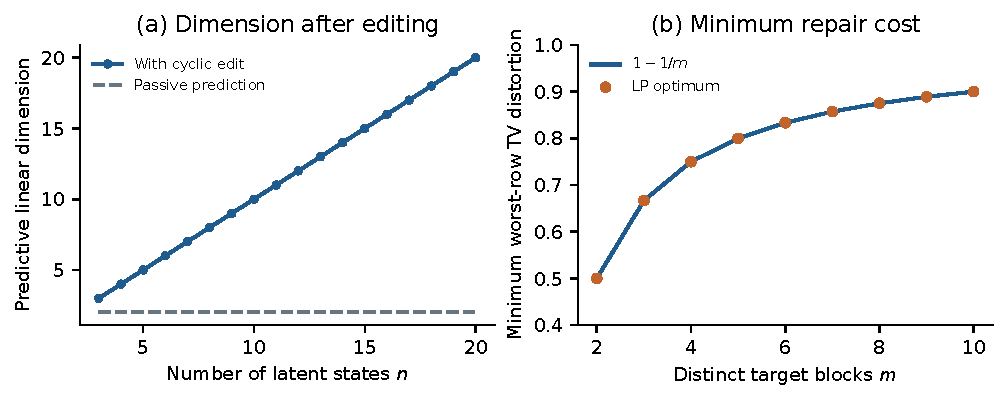
\includegraphics[width=\linewidth]{../figures/02_sharp_families.pdf}
\caption{Sharp constructed families. (a) Passive linear dimension remains two while the cyclic edit requires dimension $n$. (b) An $m$-way branching edit requires unrestricted repair cost $1-1/m$. Markers are computed LP optima; curves follow the stated formulas.}\label{fig:sharp}
\end{figure}

\section{Composition and limits of approximate prediction}
\begin{theorem}[Joint-transcript bound]\label{thm:coupling}
Compare the same finite hidden-state process with requested kernels $K_a$ and replacement kernels $L_a$ satisfying $d(K_a,L_a)\le\delta$. A controller chooses edits from observed history, using the same rule in both processes. If at most $q$ edit calls occur along each execution, then the TV distance between the joint observable transcripts is at most $1-(1-\delta)^q$. Passive observation steps may be interleaved without a fixed bound on their number, provided the transcript terminates almost surely.
\end{theorem}
\begin{proof}
Couple initial hidden states and controller randomness identically. While the hidden states and transcripts agree, the controller chooses the same edit. Couple its two transition rows maximally: disagreement probability is at most $\delta$. Couple every passive hidden-state/observation transition identically while the states agree. The probability of no disagreement through at most $q$ edit opportunities is at least $(1-\delta)^q$. The coupling inequality gives the transcript bound; almost-sure termination extends it from finite truncations.
\end{proof}
The bound is standard sequential coupling applied to edit calls. Compatibility is needed to implement a replacement on the compressed interface, but the transcript bound itself holds for any kernels satisfying the row-TV condition. It controls joint laws, not posterior laws conditioned on a rare observed event. Conditioning can amplify arbitrarily small joint differences; Appendix~\ref{app:conditioning} gives an explicit example.

\paragraph{Near-aliasing is not an approximate certificate.}
Exact rank is also insufficient as a practical diagnostic when learned models are uncertain. Consider a static four-state binary-emission model with success probabilities $(1/2-\epsilon,1/2+\epsilon,0.05,0.95)$, $0<\epsilon\le0.1$. The priors $e_1,e_2$ differ by $2\epsilon$ TV for one observation, and by at most $2T\epsilon$ for $T$ observations. An edit sending state 1 to state 3 and state 2 to state 4 makes their one-step TV distance $0.9$. Thus no vanishing bound based only on fixed-horizon passive prediction discrepancy controls every specified edit. For positive $\epsilon$ the exact passive model can have full rank; the difficulty is ill-conditioning, not exact nonidentifiability. This example does not estimate the behavior of a trained model.

\section{Computational evaluation}\label{sec:experiments}
\subsection{Protocol and independent checks}
The artifact includes source code, frozen generator settings, raw kernels, repaired kernels, dual vectors, CSV results, and scripts for figures and verification. All reported experiments were executed locally with Python 3.9.6, NumPy 1.26.4 and SciPy 1.13.1 on an ARM64 macOS host. The experiments test finite mathematical specifications; none uses a pretrained model or an external benchmark. A locally written protocol preceded the main experiment. The support extension and stronger mean-aggregate baseline were added afterward and are identified separately in the artifact. This is not an external preregistration.

\paragraph{Exact arithmetic.}
For $n=2,3,4$, enumerate all $n^n$ deterministic kernels on each of two representations: a two-block partition and a rational nonpartition encoding with two anchor rows and rational mixture rows. An independent Fraction-based Gaussian elimination checks
$\rank[O,KO]=\rank O$.
The numerical compatibility test agrees on all $2(2^2+3^3+4^4)=574$ cases. These are exhaustive checks for the declared finite set, not a proof for arbitrary real-valued inputs. Eleven unit tests additionally cover the mixture witness, reset compatibility, full representations, sharp families, support infeasibility, agreement between full and reduced repair solvers, and reuse of saved dual bases.

\paragraph{Main generators.}
We use $n\in\{6,12,18\}$, predictive rank $r\in\{2,3\}$ and 20 seeds per stratum, giving 120 partition and 120 nonpartition cases. Partition labels are balanced and permuted. For nonpartition models, an $n\times r$ matrix $E$ contains $r$ identity anchor rows and $n-r$ independent Dirichlet$(1)$ rows. Let $H$ select the anchors, so $HE=I_r$, and choose distinct $p_i$ equally spaced in $[0.15,0.85]$. Define
\begin{equation}
M_1=E\operatorname{diag}(p)H,\qquad M_0=E\operatorname{diag}(1-p)H.
\end{equation}
The partition construction uses the same formula with an anchor in each block. In both cases $\V=\col(E)$: every test lies in that space, and powers of the distinct emission probabilities span it by the Vandermonde argument. Desired kernels have independent Dirichlet$(0.3)$ rows. These controlled low-rank models deliberately expose the interface under study; they are not representative samples of deployed systems.

\paragraph{Baselines.}
Identity is a valid unrestricted fallback. For partitions, a common reconstruction baseline takes a uniform latent representative within each source block before applying $K$. We also include a stronger baseline: average the aggregate rows $p_i$ in each source block, then lift the mean aggregate distribution while preserving each original within-target-block conditional. This isolates the choice of center from unnecessary changes within target blocks. The full LP is checked against a separately implemented, smaller center LP on every partition instance. The baselines are explicit constructions, not reproductions of named neural editing methods.

\paragraph{Support extension.}
For each of the six $(n,r)$ strata, ten cases sample three allowed destinations per row, while ten include the diagonal and sample two other destinations. Desired probabilities follow Dirichlet$(0.3)$ on those three entries. All 120 cases are retained, including infeasible ones. The block-intersection feasibility test is compared with the full constrained LP; feasible optima are compared with the restricted-center LP.

\subsection{Results}
Table~\ref{tab:main} reports the main suite. The mean partition repair cost is 0.346, compared with 0.397 for the stronger mean-aggregate baseline and 0.581 for uniform reconstruction. The paired mean improvement over the stronger baseline is 0.0517, with descriptive percentile-bootstrap interval $[0.0441,0.0593]$ (4,000 resamples of the 120 paired differences). Reporting only the weaker reconstruction baseline would overstate the optimization gain. The mean nonpartition repair cost is 0.233. These magnitudes are conditional on the generators and metric, and are not estimates of real-world editing error.

\begin{table}[t]
\centering\small
\begin{tabular}{lrrrrr}
\toprule
Representation & Cases & Optimal TV & Mean-aggregate TV & Identity TV & Median ms\\\midrule
\PartitionRow
\MixtureRow
\bottomrule
\end{tabular}
\caption{Unrestricted repair suite. Costs are means of worst-row TV; runtime is the median full LP solve time on one local host. The nonpartition representation has no canonical block-mean baseline. Runtime is descriptive, not a scaling claim.}\label{tab:main}
\end{table}

The full and independent reduced solvers agree to at most $3.42\times10^{-10}$ in the partition suite. Main-suite maximum primal residual is $8.43\times10^{-10}$; maximum dual-feasibility residual is $2.05\times10^{-13}$. Replaying saved kernels and dual vectors without optimization verifies 335 feasible repairs across the main and support suites, with maximum cost--dual gap $4.22\times10^{-10}$. These are floating-point residual checks, not formal exact LP certificates.

The sparse-support extension finds 35 feasible cases out of 60 without a guaranteed diagonal and 60 out of 60 with the diagonal allowed (Table~\ref{tab:support}). The combinatorial feasibility criterion and the LP agree on every case. The mean extra cost of respecting support is 0.310 among the first regime's 35 feasible cases, and 0.364 in the second regime. These are different conditional populations; comparing their means does not isolate a causal effect of adding self-transitions. Diagonal permission guarantees feasibility because it admits the identity, but can still force substantial distortion.

\begin{table}[t]
\centering\small
\begin{tabular}{lrrr}
\toprule
Allowed-support generator & Feasible / total & Mean constrained TV & Mean added TV\\\midrule
Three random destinations & 35 / 60 & 0.758 & 0.310\\
Diagonal and two others & 60 / 60 & 0.845 & 0.364\\\bottomrule
\end{tabular}
\caption{Support-constrained extension. Costs and added costs are calculated on the feasible cases of each regime. All 25 infeasible specifications are retained and have explicit empty-intersection obstructions.}\label{tab:support}
\end{table}

\begin{figure}[t]
\centering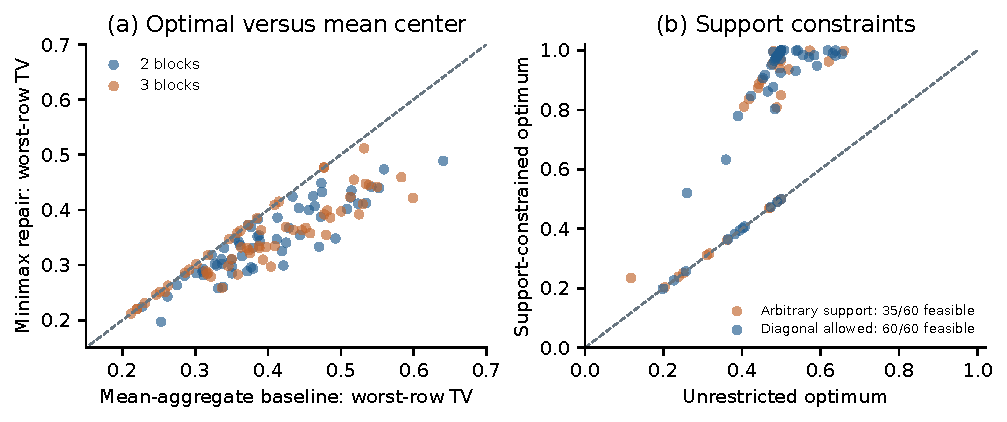
\includegraphics[width=\linewidth]{../figures/03_repair_results.pdf}
\caption{Repair comparisons. (a) Minimax center selection is compared with the stronger mean-aggregate baseline, which preserves within-target-block conditionals. (b) Respecting support raises cost on feasible instances; the other 25 arbitrary-support cases are infeasible rather than omitted numerical failures.}\label{fig:results}
\end{figure}

The 27 sharp-family instances match their analytic rank and cost formulas. In the random suite, the backward-space implementation returns edit-closed rank below $n$ in 38 of 240 cases at its $10^{-10}$ numerical threshold; all occur at $n=18,r=2$. We retain this result rather than describing all generated models as numerically full-rank. Small innovations in long products can be discarded by thresholding, so the exact dimension theorem does not turn a numerical rank estimate into a robust learned-model guarantee.

For composition, 60 generated six-state, rank-two models each supply ten fixed eight-step edit schedules. We enumerate all $2^8=256$ joint output strings per schedule. The observed transcript TV never exceeds Theorem~\ref{thm:coupling}'s bound across 600 schedules; its maximum is 0.6703. The bound is often loose (Figure~\ref{fig:composition}). The experiment checks fixed schedules, while the theorem also covers history-adaptive controllers under its assumptions. Figure~\ref{fig:composition} also plots the exact near-aliasing construction, keeping analytic curves separate from generated-model measurements.

\begin{figure}[t]
\centering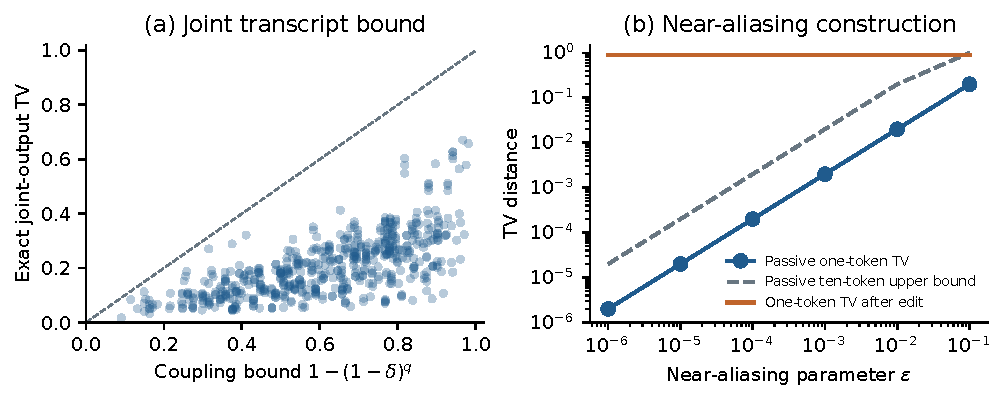
\includegraphics[width=\linewidth]{../figures/04_composition_and_conditioning.pdf}
\caption{Limits as well as guarantees. (a) Exact joint-output TV versus the coupling bound for 600 fixed schedules. The bound concerns joint transcripts, not rare-event-conditioned posteriors. (b) A stated four-state construction has arbitrarily close passive predictions while an edit separates its two priors by 0.9 TV. The ten-token passive curve is an upper bound, not a measured distance.}\label{fig:composition}
\end{figure}

\section{Implications, limitations, and next experiments}
\paragraph{A pre-edit contract.}
For an explicit finite belief module, the audit offers an actionable sequence. Declare the prediction tests, the prior domain, the edit kernel, and the transitions that may change. Test compatibility. If it fails, return contradictory priors. Then either retain the edit-closed coordinates, solve a constrained repair within an acceptable distortion budget, or reject the request. Infeasibility is useful information: silently selecting a representative belief would choose semantics not specified by the original edit.

Potential applications include simulators, structured state estimators, and model-based agent memory modules with explicit finite latent semantics. The commercial hypothesis is an audit layer for intervention interfaces, returning counterexamples and change budgets rather than only a steering score. This work does not validate customer demand, neural implementation fidelity, a patent claim, or a deployed safety benefit. A source-based tooling landscape and the additional validation needed for that hypothesis are supplied with the artifact.

\paragraph{Model-relative guarantees.}
The entire audit assumes known, correct operators. It does not identify latent causal structure from passive logs. If the model is misspecified, an exact answer can be wrong about the deployed system. Nor is an arbitrary activation patch known to induce a stochastic $K$ on the chosen beliefs. Establishing that bridge requires independent causal and distributional tests, not merely a good decoding probe. A natural follow-up is to train small transformers on the specified generators, estimate their edit maps on held-out belief mixtures, and test whether compatibility residuals predict failures under intervention. That experiment is not part of the present evidence.

\paragraph{Domain, metric, and support choices.}
Universal-prior compatibility can reject an edit that is valid on a restricted reachable set. Conversely, checking only sampled reachable beliefs can miss failures after a new edit leaves that set. The worst-row TV metric is deliberately conservative and realization-dependent. It can penalize latent changes invisible to all requested outputs. Support restrictions prevent fabricated transitions, but may make repair impossible even when an abstract output-only approximation exists. Selecting the right metric and allowed transitions is part of the application contract, not a conclusion supplied by the optimizer.

\paragraph{Numerics and scale.}
The current LP is intended for small explicit models. It has quadratic variables and dense subspace constraints in the worst case. Its millisecond runtimes at $n\le18$ do not establish large-model scalability. The numerical rank threshold is not calibrated to model-estimation uncertainty. Approximate learned representations need confidence sets, conditioning-aware guarantees, and intervention coverage; the near-aliasing example precludes replacing these with passive predictive accuracy alone.

\section{Conclusion}
Prediction sufficiency is relative to a family of tests, and a new edit can enlarge that family. For finite stochastic belief models, quotient compatibility makes this statement checkable over mixtures of priors. Fixed-interface repair can be optimized, but permitted transitions can obstruct it altogether. The restricted block-center formula, sharp constructions, and reproducible computations expose the choice facing an intervention interface: retain additional distinctions, change the requested edit under an explicit budget, or decline to implement it. Extending this contract to learned neural representations remains a concrete research task.

\paragraph{Code and results.}
\url{https://github.com/shi1720/belief-edit-audit}. The repository contains all generators, results, verification code, figures, and the manuscript source. The supplied executable checks support the finite-model claims above; there is no claim of neural-model certification.

\bibliographystyle{plainnat}
\bibliography{references}

\clearpage\appendix
\section{Implementing the compatibility audit}
Let $U$ be an orthonormal basis for $\V$. The numerical residual is
\begin{equation}
\rho(K,U)=\|(I-UU^\top)KU\|_2.
\end{equation}
In exact arithmetic it is zero exactly when compatibility holds. In floating-point arithmetic its size is descriptive unless a model-error scale is available. If a supplied test column $o_j$ has nonzero residual $v=(I-UU^\top)Ko_j$, regard $v^\top$ as a row. Then $v^\top O=0$ and
$v^\top K o_j=\|v\|_2^2>0$.
Separating positive and negative entries gives the two priors of Theorem~\ref{thm:compat}. For floating-point witnesses, both prior equality and edited separation must be checked numerically.

The backward-space routine begins with $\one$, tries operator images of accepted test columns, and keeps independent columns using twice-repeated modified Gram--Schmidt. It stops when no new column is accepted or rank reaches $n$. Its $10^{-10}$ threshold is relative to $\max(1,\|v\|_2)$. Raw test products can become small; this explains why reported numerical rank is not treated as an exact invariant. The rational exhaustive test uses a separate elimination implementation and avoids this issue on its declared small inputs.

\section{LP verification and blockwise lifting}
Write the LP in the form
$\min c^\top x$ subject to $Ax\le b$, $Bx=e$, and $x\ge0$.
For dual vectors $z\le0$ and unrestricted $y$, dual feasibility is
$c-A^\top z-B^\top y\ge0$.
The lower objective is $b^\top z+e^\top y$. The artifact stores the matrices $K,O$, support masks when supplied, repaired kernels, the solver's dual vectors, and the numerical bases used to construct its constraints. Saving the bases avoids dependence on SVD signs or null-space rotations across machines. The verifier independently checks their orthonormality, dimensions, and span, then reconstructs the constraints and checks stochasticity, compatibility, support, dual feasibility, and agreement of the dual objective with the independently recomputed worst-row TV cost. It does not trust a solver success flag as proof of validity.

The reduced partition LP uses variables $q_h$, $a_{ih}$, and $t$ for each source block. It imposes $q\ge0$, $\sum_hq_h=1$, $q_h=0$ for $h\notin J_g$, $a_{ih}\ge\pm(p_i(h)-q_h)$ and $\sum_h a_{ih}\le2t$. This implementation does not call the full repair solver. The lifting formula, where $p_i(h)>0$, is
\begin{equation}
L_{ij}=q_g(h)\,K_{ij}/p_i(h),\qquad i\in G_g,\ j\in G_h.
\end{equation}
When $p_i(h)=0$, choose any supported distribution in $G_h$ if $q_g(h)>0$. This also shows why the assumption $\operatorname{supp}(K)\subseteq S$ matters for the support-constrained equality: otherwise preserving the original conditional could retain forbidden entries.

\section{Restricted prior domains}\label{app:domains}
Suppose permitted input beliefs form $\mathcal B=\operatorname{conv}\{f_1,\ldots,f_k\}$, and stack its vertices as rows of $F\in\mathbb R^{k\times n}$. The edit has a well-defined predictive effect on this domain exactly when
\begin{equation}
\ker_{\mathrm{row}}(FO)\subseteq\ker_{\mathrm{row}}(FKO),
\quad\text{equivalently}\quad
\rank[FO,FKO]=\rank(FO).
\end{equation}
To see necessity, take a row $\alpha$ annihilating $FO$. Since $\one$ is represented and every $f_i$ is normalized, $\alpha\one=0$. Its positive and negative parts, normalized by their common mass, define two convex combinations of rows of $F$ with the same prediction. Domain compatibility requires their edited predictions to agree, so $\alpha FKO=0$. The converse follows by taking the difference of any two coefficient vectors representing beliefs with equal $FO$ coordinates.

This criterion concerns one edit at one domain. A compositional guarantee requires the domain to include beliefs reached after subsequent edits and normalized observation updates. A singleton prior domain makes the one-edit criterion vacuous, illustrating why domain declaration is material. The released repair experiments use the universal domain $F=I$; no empirical claim is made for estimating a reachable-domain polytope.

\section{Why conditioning needs a separate bound}\label{app:conditioning}
Let transcripts take values $\{a,b,c\}$. For $0<\eta<1$, let $P(a)=\eta$, $P(b)=0$, $P(c)=1-\eta$, while $Q(a)=0$, $Q(b)=\eta$, $Q(c)=1-\eta$. Then $\TV(P,Q)=\eta$. On the event $A=\{a,b\}$, both laws assign probability $\eta$, but their conditional distributions have TV one. Consequently an arbitrarily small joint-law guarantee does not certify a small posterior discrepancy on every event. Theorem~\ref{thm:coupling} intentionally makes no such claim.

For the near-aliasing construction, couple Bernoulli observations with probabilities $1/2-\epsilon$ and $1/2+\epsilon$ using the same uniform variate at every step. Each step disagrees with probability $2\epsilon$, so the TV of length-$T$ traces is at most $1-(1-2\epsilon)^T\le2T\epsilon$. Mapping the priors to states with emission probabilities 0.05 and 0.95 makes the edited one-step TV exactly 0.9. This is the source of Figure~\ref{fig:composition}(b).

\section{Reproduction map}
From the repository root, install the pinned requirements and run:
\begin{verbatim}
python3 -m unittest discover -s tests -v
OPENBLAS_NUM_THREADS=1 python3 experiments/run.py
OPENBLAS_NUM_THREADS=1 python3 experiments/support.py
OPENBLAS_NUM_THREADS=1 python3 experiments/augment_and_verify.py
python3 experiments/figures.py
cd paper
tectonic main.tex
\end{verbatim}
The generated \texttt{main.csv} has 240 rows; \texttt{support.csv} has 120; \texttt{composition.csv} has 600; and \texttt{sharp.csv} has 27. Runtime will vary. All kernel costs and figures are regenerated from the stated seeds or explicit formulas. The support extension and added baseline are documented as post-main-run analyses. The artifact's literature matrix records the primary sources and the bounded novelty assessment.
\end{document}
